\documentclass[tikz]{article}
\usepackage[utf8]{inputenc}
\usepackage[tmargin=2in]{geometry}
\usepackage{setspace}
\usepackage{verbatim}
\usepackage{listings}
\usepackage{amsmath}
\usepackage{amssymb}
\usepackage{pgfplots}
\usepackage{graphics}
\usepackage{csvsimple}
\usepackage{array}
\usepackage{longtable}
\usepackage{booktabs}
\usepackage{pgfplotstable}
\usepackage[toc,page]{appendix}
\usepackage{indentfirst}
\usepackage{float}
\usepackage{setspace}
\usepackage{multirow}
\usepackage{tikz}
\usetikzlibrary{positioning}

\newcommand\MyBox[2]{
  \fbox{\lower0.75cm
    \vbox to 1.7cm{\vfil
      \hbox to 1.7cm{\hfil\parbox{1.4cm}{#1}\hfil}
      \vfil}%
  }%
}


\doublespacing
\pagenumbering{gobble}

\pgfplotsset{every axis/.style={scale only axis}}

\begin{document}

\begin{center}
Dustin McAfee \\
Project 4 Report \\
Fall 2018 \\
\end{center}

\singlespacing

\section{Objective}
\label{sec:obj}
There is a dataset of email attributes, 4601 observations each with 55 continuous real attributes, 2 continuous integer attributes, and one binary categorical attribute. The objective is to predict the binary categorical attribute, 'Spam', by training an online artificial neural network with a softmax output layer. There are many hyper-parameters to tune: learning rate, number of neurons per hidden layer, and number of hidden layers. Average performance metrics such as confusion matrices and F1 scores are computed and shown for different K-Fold cross-validations of these hyper-parameters. The optimal hyper-parameters are chosen and run on the testing dataset and the performance metrics are shown. PCA is also performed on the entire dataset to reduce the dimensions in an attempt to increase the neural network performance on the testing dataset. 

\section{Data Preprocessing}
\label{sec:preprocessing}
There are no missing values from the data, and 58 total dimensions (57 not including the binary categorical attribute). The last column of the dataset represents the categorical attribute, and the rest of the columns are z-normalized. The dataset is split into separate testing and training datasets, in which the testing dataset represents about 13\% (600) of all observations (See files "TestingData.txt" and "TrainingData.txt").


\section{Methods}
\label{sec:methods}
K-fold cross validation is implemented and performed with 5 groups (folds) of training sets (See function "n\_fold\_split" in "net.py"). Each K-fold cross-validation training set has about 920 observations, which correspond to about 3680 observations for validation of each K-fold. The artificial neural network is tuned for the learning rate, number of neurons per hidden layer, and number of hidden layers. For each one of these hyper-parameters being cross-validated, the others are held constant. The maximum number of epochs is always held constant at 1000 (since each K-fold of the training data takes several minutes with this many epochs, this number seemed like a practical maximum), and the cutoff tolerance for the sum of squared errors for the output of each epoch is 0.001. The error is printed to screen for each 10 epochs, and a keyboard interrupt continues from the back propagation loop. While cross-validating, the learning rate is held at 0.1, the number of neurons per hidden layer is held at 3, and the number of hidden layers is held at 2. The first hyper-parameter tuned is the learning rate, which is tested from 0.01, 0.1, 0.2, 0.3,  and 0.5. Then, the number of neurons per hidden layer, which is tested in the range of 1 to 6. Last, is the number of hidden layers, which is tested in the range of 1 to 5 (2 to 6 total layers, including the output layer). A confusion matrix is shown from the average performance metrics of the K-fold cross-validation datasets for each hyper-parameter. A final confusion matrix is produced for the testing dataset with the chosen optimal hyper-parameters. \\

\subsection{Learning Rate}
\label{sec:hyper1}
For a learning rate of 0.01, the average of the 5 folds yields 80.17\% accuracy, with 57.02\% sensitivity, 88.58\% precision, 95.19\% specificity, and a F1 score of 69.20\%. The average sum of squared errors for the output of each K-fold is 369.79 after each fold reaches 1000 epochs. The confusion matrix for this is shown below, in Figure \ref{fig:l01}.


\begin{figure}[H]
\begin{center}
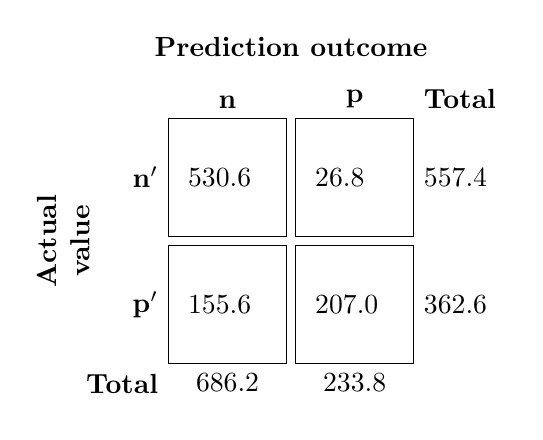
\begin{tikzpicture}[
box/.style={draw,rectangle,minimum size=1.5cm,text width=1.0cm,align=left}]
\matrix (conmat) [row sep=.1cm,column sep=.1cm] {
\node (tneg) [box,
    label=left:\( \mathbf{n'} \),
    label=above:\( \mathbf{n} \),
    ] {530.6};
&

\node (fpos) [box,
    label=above:\textbf{p},
    label=above right:\textbf{Total},
    label=right:\( \mathrm{557.4} \)] {26.8};
\\
\node (fneg) [box,
    label=left:\( \mathbf{p'} \),
    label=below left:\textbf{Total},
    label=below:686.2] {155.6};
&
\node (tpos) [box,
    label=right:\( \mathrm{362.6} \),
    label=below:233.8] {207.0};
\\
};
\node [rotate=90,left=.05cm of conmat,anchor=center,text width=1.5cm,align=center] {\textbf{Actual \\ value}};
\node [above=.05cm of conmat] {\textbf{Prediction outcome}};
\end{tikzpicture}
\caption{Confusion Matrix for Learning Rate = 0.01}
\label{fig:l01}
\end{center}
\end{figure}

This has a very high false negative rate, and a rather too high false positive rate. During this run, the sum of squared errors monotonically decreases. Because of this, it is likely, that if the neural network is trained for a longer time (more epochs), then there would be a better fit for this data. Unfortunately, more epochs are not practical given the complexity of the algorithm (See file "net.py"). \\

For a learning rate of 0.1, the average of the 5 folds yields 78.63\% accuracy, with 50.25\% sensitivity, 91.74\% precision, 97.01\% specificity, and a F1 score of 64.71\%. The average sum of squared errors for the output of each K-fold is 382.72 after each fold reaches 1000 epochs. The confusion matrix for this is shown below, in Figure \ref{fig:l1}.


\begin{figure}[H]
\begin{center}
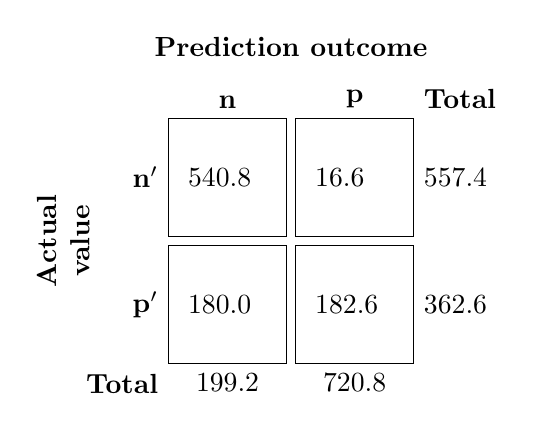
\begin{tikzpicture}[
box/.style={draw,rectangle,minimum size=1.5cm,text width=1.0cm,align=left}]
\matrix (conmat) [row sep=.1cm,column sep=.1cm] {
\node (tneg) [box,
    label=left:\( \mathbf{n'} \),
    label=above:\( \mathbf{n} \),
    ] {540.8};
&

\node (fpos) [box,
    label=above:\textbf{p},
    label=above right:\textbf{Total},
    label=right:\( \mathrm{557.4} \)] {16.6};
\\
\node (fneg) [box,
    label=left:\( \mathbf{p'} \),
    label=below left:\textbf{Total},
    label=below:199.2] {180.0};
&
\node (tpos) [box,
    label=right:\( \mathrm{362.6} \),
    label=below:720.8] {182.6};
\\
};
\node [rotate=90,left=.05cm of conmat,anchor=center,text width=1.5cm,align=center] {\textbf{Actual \\ value}};
\node [above=.05cm of conmat] {\textbf{Prediction outcome}};
\end{tikzpicture}
\caption{Confusion Matrix for Learning Rate = 0.1}
\label{fig:l1}
\end{center}
\end{figure}

This run has less false positives, which means there are less important emails that are misclassified as spam. It has slightly less accuracy, less sensitivity, but higher precision and specificity. Like the last architecture, the sum of squared errors monotonically decreased during the entire execution on this dataset. \\

For a learning rate of 0.2, the average of the 5 folds yields 79.02\% accuracy, with 51.61\% sensitivity, 91.29\% precision, 96.80\% specificity, and a F1 score of 65.85\%. The average sum of squared errors for the output of each K-fold is 406.40 after each fold reaches 1000 epochs. The confusion matrix for this is shown below, in Figure \ref{fig:l2}.


\begin{figure}[H]
\begin{center}
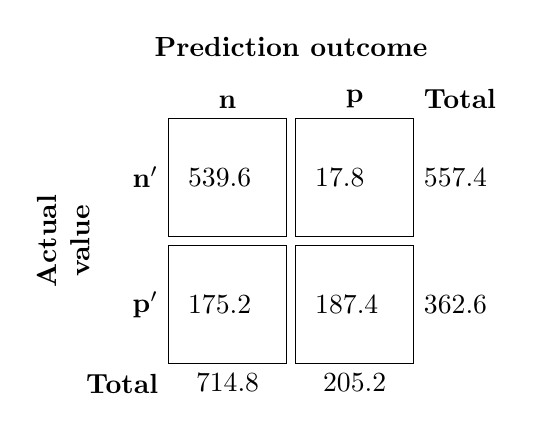
\begin{tikzpicture}[
box/.style={draw,rectangle,minimum size=1.5cm,text width=1.0cm,align=left}]
\matrix (conmat) [row sep=.1cm,column sep=.1cm] {
\node (tneg) [box,
    label=left:\( \mathbf{n'} \),
    label=above:\( \mathbf{n} \),
    ] {539.6};
&

\node (fpos) [box,
    label=above:\textbf{p},
    label=above right:\textbf{Total},
    label=right:\( \mathrm{557.4} \)] {17.8};
\\
\node (fneg) [box,
    label=left:\( \mathbf{p'} \),
    label=below left:\textbf{Total},
    label=below:714.8] {175.2};
&
\node (tpos) [box,
    label=right:\( \mathrm{362.6} \),
    label=below:205.2] {187.4};
\\
};
\node [rotate=90,left=.05cm of conmat,anchor=center,text width=1.5cm,align=center] {\textbf{Actual \\ value}};
\node [above=.05cm of conmat] {\textbf{Prediction outcome}};
\end{tikzpicture}
\caption{Confusion Matrix for Learning Rate = 0.2}
\label{fig:l2}
\end{center}
\end{figure}

For a learning rate of 0.3, the average of the 5 folds yields 78.28\% accuracy, with 50.16\% sensitivity, 90.44\% precision, 96.51\% specificity, and a F1 score of 64.35\%. The average sum of squared errors for the output of each K-fold is 437.23 after each fold reaches 1000 epochs. The confusion matrix for this is shown below, in Figure \ref{fig:l3}.


\begin{figure}[H]
\begin{center}
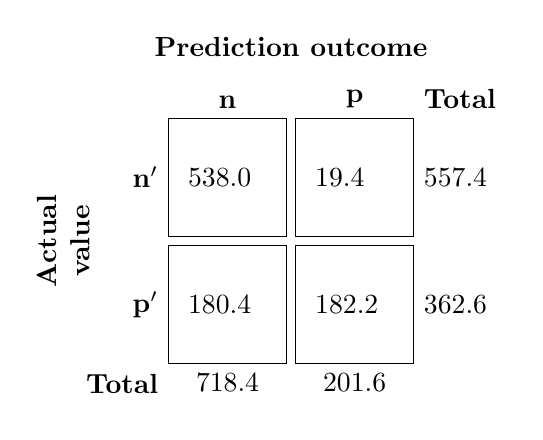
\begin{tikzpicture}[
box/.style={draw,rectangle,minimum size=1.5cm,text width=1.0cm,align=left}]
\matrix (conmat) [row sep=.1cm,column sep=.1cm] {
\node (tneg) [box,
    label=left:\( \mathbf{n'} \),
    label=above:\( \mathbf{n} \),
    ] {538.0};
&

\node (fpos) [box,
    label=above:\textbf{p},
    label=above right:\textbf{Total},
    label=right:\( \mathrm{557.4} \)] {19.4};
\\
\node (fneg) [box,
    label=left:\( \mathbf{p'} \),
    label=below left:\textbf{Total},
    label=below:718.4] {180.4};
&
\node (tpos) [box,
    label=right:\( \mathrm{362.6} \),
    label=below:201.6] {182.2};
\\
};
\node [rotate=90,left=.05cm of conmat,anchor=center,text width=1.5cm,align=center] {\textbf{Actual \\ value}};
\node [above=.05cm of conmat] {\textbf{Prediction outcome}};
\end{tikzpicture}
\caption{Confusion Matrix for Learning Rate = 0.3}
\label{fig:l3}
\end{center}
\end{figure}

For a learning rate of 0.5, the average of the 5 folds yields 70.48\% accuracy, with 27.71\% sensitivity, 90.55\% precision, 98.09\% specificity, and a F1 score of 42.43\%. The average sum of squared errors for the output of each K-fold is 509.11 after each fold reaches 1000 epochs. The confusion matrix for this is shown below, in Figure \ref{fig:l5}.


\begin{figure}[H]
\begin{center}
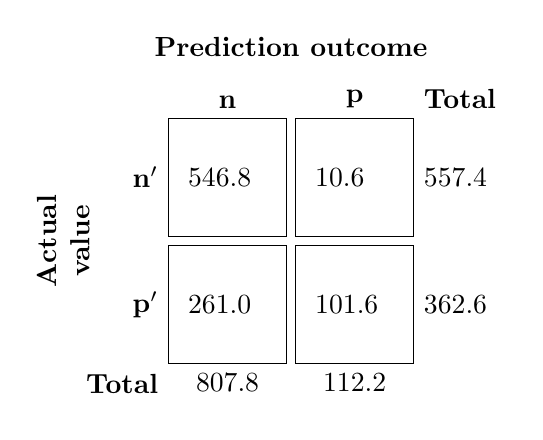
\begin{tikzpicture}[
box/.style={draw,rectangle,minimum size=1.5cm,text width=1.0cm,align=left}]
\matrix (conmat) [row sep=.1cm,column sep=.1cm] {
\node (tneg) [box,
    label=left:\( \mathbf{n'} \),
    label=above:\( \mathbf{n} \),
    ] {546.8};
&

\node (fpos) [box,
    label=above:\textbf{p},
    label=above right:\textbf{Total},
    label=right:\( \mathrm{557.4} \)] {10.6};
\\
\node (fneg) [box,
    label=left:\( \mathbf{p'} \),
    label=below left:\textbf{Total},
    label=below:807.8] {261.0};
&
\node (tpos) [box,
    label=right:\( \mathrm{362.6} \),
    label=below:112.2] {101.6};
\\
};
\node [rotate=90,left=.05cm of conmat,anchor=center,text width=1.5cm,align=center] {\textbf{Actual \\ value}};
\node [above=.05cm of conmat] {\textbf{Prediction outcome}};
\end{tikzpicture}
\caption{Confusion Matrix for Learning Rate = 0.5}
\label{fig:l5}
\end{center}
\end{figure}

The optimal learning rate chosen is 0.1, since, other than with a learning rate of 0.5, it has the lowest false positive rate with better performance metrics than most of the others (though it is very close to the learning rate of 0.01 with a slightly higher accuracy and precision). It is important to note, that each execution of the neural network with variable learning rates monotonically decreased and did not necessarily converge to a specific sum of squared errors value (See files "l\_rate\_01," "l\_rate\_1," "l\_rate\_2," "l\_rate\_3," "l\_rate\_5," and "l\_rate\_8").

\subsection{Number of Neurons per Hidden Layer}
\label{sec:hyper2}
In this subsection, the hyper-parameter tuned is the number of neurons per hidden layer. Recall that for cross-validation, the other hyper-parameters are held constant, and the number of hidden layers is held at 2. For 1 neuron per hidden layer, the average of the 5 folds yields 80.39\% accuracy, with 55.55\% sensitivity, 91.27\% precision, 96.52\% specificity, and a F1 score of 69.01\%. The average sum of squared errors for the output of each K-fold is 392.74 after each fold reaches 1000 epochs. The confusion matrix for this is shown below, in Figure \ref{fig:nn1}.


\begin{figure}[H]
\begin{center}
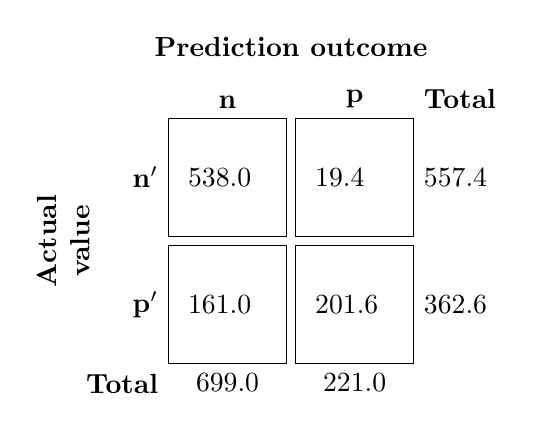
\begin{tikzpicture}[
box/.style={draw,rectangle,minimum size=1.5cm,text width=1.0cm,align=left}]
\matrix (conmat) [row sep=.1cm,column sep=.1cm] {
\node (tneg) [box,
    label=left:\( \mathbf{n'} \),
    label=above:\( \mathbf{n} \),
    ] {538.0};
&

\node (fpos) [box,
    label=above:\textbf{p},
    label=above right:\textbf{Total},
    label=right:\( \mathrm{557.4} \)] {19.4};
\\
\node (fneg) [box,
    label=left:\( \mathbf{p'} \),
    label=below left:\textbf{Total},
    label=below:699.0] {161.0};
&
\node (tpos) [box,
    label=right:\( \mathrm{362.6} \),
    label=below:221.0] {201.6};
\\
};
\node [rotate=90,left=.05cm of conmat,anchor=center,text width=1.5cm,align=center] {\textbf{Actual \\ value}};
\node [above=.05cm of conmat] {\textbf{Prediction outcome}};
\end{tikzpicture}
\caption{Confusion Matrix for Number of Neurons per Hidden Layer = 1}
\label{fig:nn1}
\end{center}
\end{figure}

For 2 neurons per hidden layer, the average of the 5 folds yields 79.65\% accuracy, with 53.39\% sensitivity, 91.35\% precision, 96.65\% specificity, and a F1 score of 67.10\%. The average sum of squared errors for the output of each K-fold is 385.92 after each fold reaches 1000 epochs. The confusion matrix for this is shown below, in Figure \ref{fig:nn2}.


\begin{figure}[H]
\begin{center}
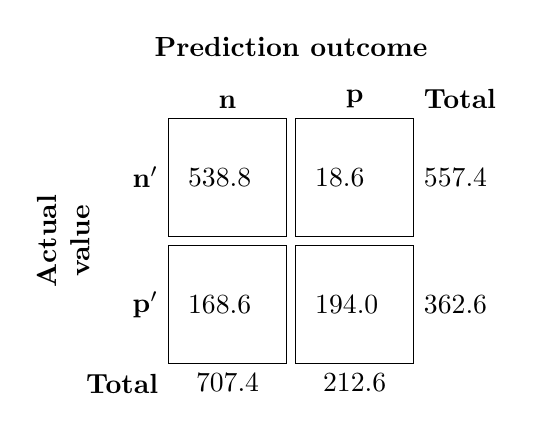
\begin{tikzpicture}[
box/.style={draw,rectangle,minimum size=1.5cm,text width=1.0cm,align=left}]
\matrix (conmat) [row sep=.1cm,column sep=.1cm] {
\node (tneg) [box,
    label=left:\( \mathbf{n'} \),
    label=above:\( \mathbf{n} \),
    ] {538.8};
&

\node (fpos) [box,
    label=above:\textbf{p},
    label=above right:\textbf{Total},
    label=right:\( \mathrm{557.4} \)] {18.6};
\\
\node (fneg) [box,
    label=left:\( \mathbf{p'} \),
    label=below left:\textbf{Total},
    label=below:707.4] {168.6};
&
\node (tpos) [box,
    label=right:\( \mathrm{362.6} \),
    label=below:212.6] {194.0};
\\
};
\node [rotate=90,left=.05cm of conmat,anchor=center,text width=1.5cm,align=center] {\textbf{Actual \\ value}};
\node [above=.05cm of conmat] {\textbf{Prediction outcome}};
\end{tikzpicture}
\caption{Confusion Matrix for Number of Neurons per Hidden Layer = 2}
\label{fig:nn2}
\end{center}
\end{figure}

For 3 neurons per hidden layer, refer back to Figure \ref{fig:l1} in Section \ref{sec:hyper1}. For 4 neurons per hidden layer, the average of the 5 folds yields 78.87\% accuracy, with 51.03\% sensitivity, 91.57\% precision, 96.90\% specificity, and a F1 score of 65.33\%. The average sum of squared errors for the output of each K-fold is 381.74 after each fold reaches 1000 epochs. The confusion matrix for this is shown below, in Figure \ref{fig:nn4}.


\begin{figure}[H]
\begin{center}
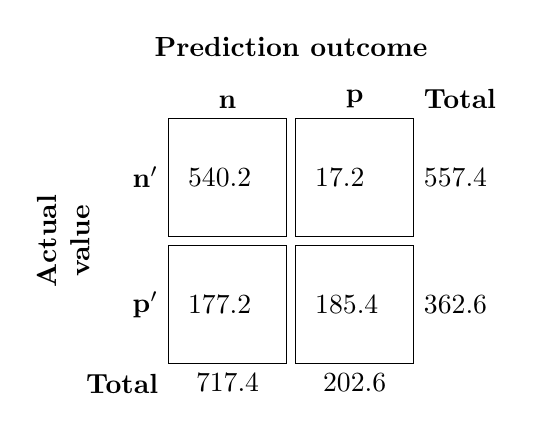
\begin{tikzpicture}[
box/.style={draw,rectangle,minimum size=1.5cm,text width=1.0cm,align=left}]
\matrix (conmat) [row sep=.1cm,column sep=.1cm] {
\node (tneg) [box,
    label=left:\( \mathbf{n'} \),
    label=above:\( \mathbf{n} \),
    ] {540.2};
&

\node (fpos) [box,
    label=above:\textbf{p},
    label=above right:\textbf{Total},
    label=right:\( \mathrm{557.4} \)] {17.2};
\\
\node (fneg) [box,
    label=left:\( \mathbf{p'} \),
    label=below left:\textbf{Total},
    label=below:717.4] {177.2};
&
\node (tpos) [box,
    label=right:\( \mathrm{362.6} \),
    label=below:202.6] {185.4};
\\
};
\node [rotate=90,left=.05cm of conmat,anchor=center,text width=1.5cm,align=center] {\textbf{Actual \\ value}};
\node [above=.05cm of conmat] {\textbf{Prediction outcome}};
\end{tikzpicture}
\caption{Confusion Matrix for Number of Neurons per Hidden Layer = 4}
\label{fig:nn4}
\end{center}
\end{figure}

For 5 neurons per hidden layer, the average of the 5 folds yields 79.15\% accuracy, with 51.88\% sensitivity, 91.46\% precision, 96.83\% specificity, and a F1 score of 66.06\%. The average sum of squared errors for the output of each K-fold is 382.70 after each fold reaches 1000 epochs. The confusion matrix for this is shown below, in Figure \ref{fig:nn5}.


\begin{figure}[H]
\begin{center}
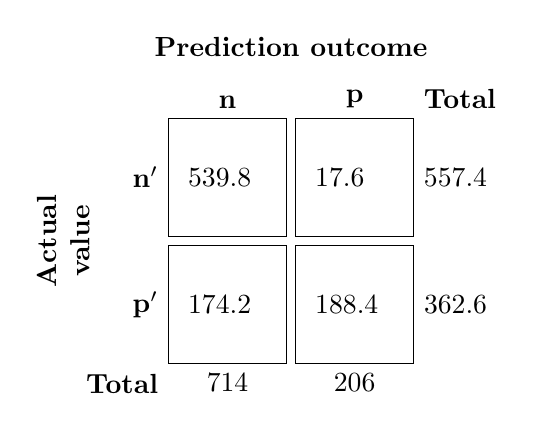
\begin{tikzpicture}[
box/.style={draw,rectangle,minimum size=1.5cm,text width=1.0cm,align=left}]
\matrix (conmat) [row sep=.1cm,column sep=.1cm] {
\node (tneg) [box,
    label=left:\( \mathbf{n'} \),
    label=above:\( \mathbf{n} \),
    ] {539.8};
&

\node (fpos) [box,
    label=above:\textbf{p},
    label=above right:\textbf{Total},
    label=right:\( \mathrm{557.4} \)] {17.6};
\\
\node (fneg) [box,
    label=left:\( \mathbf{p'} \),
    label=below left:\textbf{Total},
    label=below:714] {174.2};
&
\node (tpos) [box,
    label=right:\( \mathrm{362.6} \),
    label=below:206] {188.4};
\\
};
\node [rotate=90,left=.05cm of conmat,anchor=center,text width=1.5cm,align=center] {\textbf{Actual \\ value}};
\node [above=.05cm of conmat] {\textbf{Prediction outcome}};
\end{tikzpicture}
\caption{Confusion Matrix for Number of Neurons per Hidden Layer = 5}
\label{fig:nn5}
\end{center}
\end{figure}

For 6 neurons per hidden layer, the average of the 5 folds yields 79.17\% accuracy, with 52.20\% sensitivity, 91.07\% precision, 96.66\% specificity, and a F1 score of 66.20\%. The average sum of squared errors for the output of each K-fold is 382.93 after each fold reaches 1000 epochs. The confusion matrix for this is shown below, in Figure \ref{fig:nn6}.


\begin{figure}[H]
\begin{center}
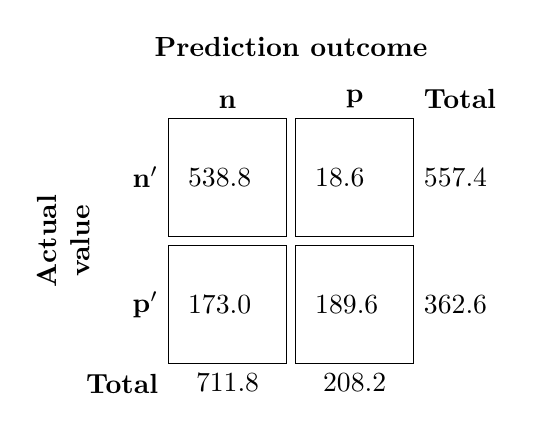
\begin{tikzpicture}[
box/.style={draw,rectangle,minimum size=1.5cm,text width=1.0cm,align=left}]
\matrix (conmat) [row sep=.1cm,column sep=.1cm] {
\node (tneg) [box,
    label=left:\( \mathbf{n'} \),
    label=above:\( \mathbf{n} \),
    ] {538.8};
&

\node (fpos) [box,
    label=above:\textbf{p},
    label=above right:\textbf{Total},
    label=right:\( \mathrm{557.4} \)] {18.6};
\\
\node (fneg) [box,
    label=left:\( \mathbf{p'} \),
    label=below left:\textbf{Total},
    label=below:711.8] {173.0};
&
\node (tpos) [box,
    label=right:\( \mathrm{362.6} \),
    label=below:208.2] {189.6};
\\
};
\node [rotate=90,left=.05cm of conmat,anchor=center,text width=1.5cm,align=center] {\textbf{Actual \\ value}};
\node [above=.05cm of conmat] {\textbf{Prediction outcome}};
\end{tikzpicture}
\caption{Confusion Matrix for Number of Neurons per Hidden Layer = 6}
\label{fig:nn6}
\end{center}
\end{figure}

The metrics in this section do not vary much; there is not much significance in the difference in performance. So, the optimal parameter value chosen here is 3 neurons per hidden layer, since part of the goal here is to have a simple predictive model, and with 3 neurons per hidden layer, the performance metrics yields the lowest false positive rate.

\subsection{Number of Hidden Layers}
\label{sec:hyper3}
In this subsection, the final hyper-parameter is tuned: The number of hidden layers. Recall, the number of neurons per hidden layer is held at 3. For 1 hidden layer, the average of the 5 folds yields 75.91\% accuracy, with 44.01\% sensitivity, 89.08\% precision, 96.41\% specificity, and a F1 score of 58.11\%. The average sum of squared errors for the output of each K-fold is 462.72 after each fold reaches 1000 epochs. The confusion matrix for this is shown below, in Figure \ref{fig:nhl1}.

\begin{figure}[H]
\begin{center}
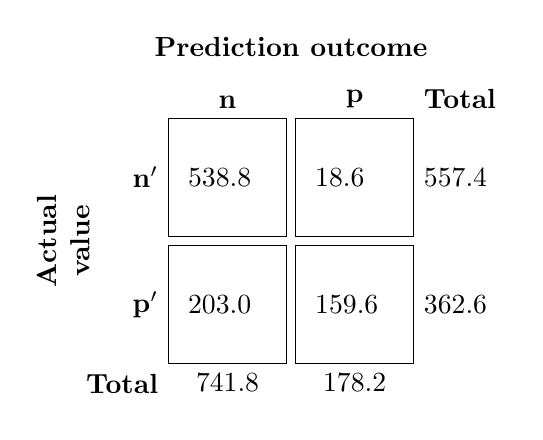
\begin{tikzpicture}[
box/.style={draw,rectangle,minimum size=1.5cm,text width=1.0cm,align=left}]
\matrix (conmat) [row sep=.1cm,column sep=.1cm] {
\node (tneg) [box,
    label=left:\( \mathbf{n'} \),
    label=above:\( \mathbf{n} \),
    ] {538.8};
&

\node (fpos) [box,
    label=above:\textbf{p},
    label=above right:\textbf{Total},
    label=right:\( \mathrm{557.4} \)] {18.6};
\\
\node (fneg) [box,
    label=left:\( \mathbf{p'} \),
    label=below left:\textbf{Total},
    label=below:741.8] {203.0};
&
\node (tpos) [box,
    label=right:\( \mathrm{362.6} \),
    label=below:178.2] {159.6};
\\
};
\node [rotate=90,left=.05cm of conmat,anchor=center,text width=1.5cm,align=center] {\textbf{Actual \\ value}};
\node [above=.05cm of conmat] {\textbf{Prediction outcome}};
\end{tikzpicture}
\caption{Confusion Matrix for Number of Hidden Layers = 1}
\label{fig:nhl1}
\end{center}
\end{figure}

For 2 hidden layers, refer back to Figure \ref{fig:l1} in Section \ref{sec:hyper1}. For 3 hidden layers, the average of the 5 folds yields 80.28\% accuracy, with 56.51\% sensitivity, 89.64\% precision, 95.68\% specificity, and a F1 score of 69.22\%. The average sum of squared errors for the output of each K-fold is 402.96 after each fold reaches 1000 epochs. The confusion matrix for this is shown below, in Figure \ref{fig:nhl3}.


\begin{figure}[H]
\begin{center}
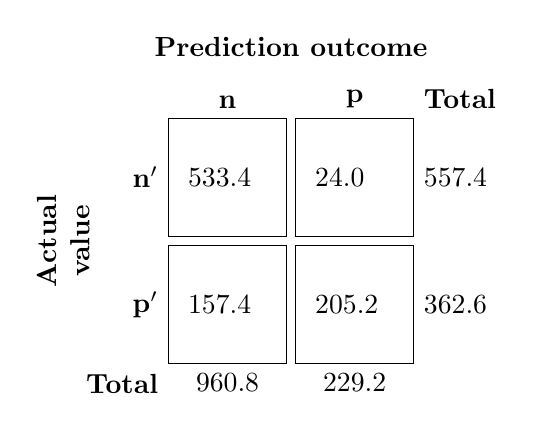
\begin{tikzpicture}[
box/.style={draw,rectangle,minimum size=1.5cm,text width=1.0cm,align=left}]
\matrix (conmat) [row sep=.1cm,column sep=.1cm] {
\node (tneg) [box,
    label=left:\( \mathbf{n'} \),
    label=above:\( \mathbf{n} \),
    ] {533.4};
&

\node (fpos) [box,
    label=above:\textbf{p},
    label=above right:\textbf{Total},
    label=right:\( \mathrm{557.4} \)] {24.0};
\\
\node (fneg) [box,
    label=left:\( \mathbf{p'} \),
    label=below left:\textbf{Total},
    label=below:960.8] {157.4};
&
\node (tpos) [box,
    label=right:\( \mathrm{362.6} \),
    label=below:229.2] {205.2};
\\
};
\node [rotate=90,left=.05cm of conmat,anchor=center,text width=1.5cm,align=center] {\textbf{Actual \\ value}};
\node [above=.05cm of conmat] {\textbf{Prediction outcome}};
\end{tikzpicture}
\caption{Confusion Matrix for Number of Hidden Layers = 3}
\label{fig:nhl3}
\end{center}
\end{figure}

For 4 or more hidden layers, the sum of squared errors for the output of each epoch quickly converges to a high number (around 930 to 1000), and the accuracy drops to 50\% or below. The confusion matrices and exact metrics for 4 and 5 hidden layers are not shown here, as it suffices to say that they do not perform well. To this end, the optimal value for the number of hidden layers is chosen to be 3. The performance metrics between, 2 and 3 hidden layers are very similar, but 3 is chosen for having higher accuracy and sensitivity, and a lower false positive rate. 


\section{Testing Dataset and Principal Component Analysis}
\label{sec:pca}
The optimal hyper-parameters are chosen from the previous section and run on the testing dataset. These values are 0.1 learning rate, 2 hidden layers, and 3 neurons per hidden layer (See Figure \ref{fig:l1} in Section \ref{sec:hyper1} for metrics on the training dataset). The network is trained on the training dataset and the testing dataset is propagated forward through the neural network to make predictions. This run yields 86.67\% accuracy, with 94.98\% sensitivity, 76.95\% precision, 81.16\% specificity, and a F1 score of 85.02\%. The sum of squared errors for the output is 401.02 after 1000 epochs. The confusion matrix for this is shown below, in Figure \ref{fig:test}.

\begin{figure}[H]
\begin{center}
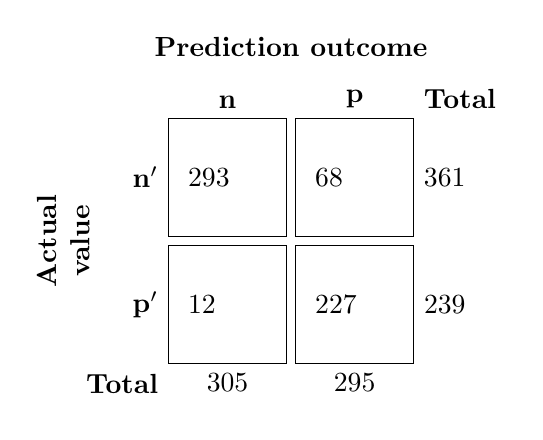
\begin{tikzpicture}[
box/.style={draw,rectangle,minimum size=1.5cm,text width=1.0cm,align=left}]
\matrix (conmat) [row sep=.1cm,column sep=.1cm] {
\node (tneg) [box,
    label=left:\( \mathbf{n'} \),
    label=above:\( \mathbf{n} \),
    ] {293};
&

\node (fpos) [box,
    label=above:\textbf{p},
    label=above right:\textbf{Total},
    label=right:\( \mathrm{361} \)] {68};
\\
\node (fneg) [box,
    label=left:\( \mathbf{p'} \),
    label=below left:\textbf{Total},
    label=below:305] {12};
&
\node (tpos) [box,
    label=right:\( \mathrm{239} \),
    label=below:295] {227};
\\
};
\node [rotate=90,left=.05cm of conmat,anchor=center,text width=1.5cm,align=center] {\textbf{Actual \\ value}};
\node [above=.05cm of conmat] {\textbf{Prediction outcome}};
\end{tikzpicture}
\caption{Confusion Matrix for Testing Dataset}
\label{fig:test}
\end{center}
\end{figure}


This seems to have a higher false positive rate than foreseen, but the overall metrics of this is much higher than that of the training dataset. \\

Principal component analysis is performed to reduce the data to a few dimensions in an attempt to increase performance. The first three principal components cover about 99.99\% of the variance of the dataset, and so, the testing dataset is projected to the first three principal components. The optimal hyper-parameters are chosen to run the neural network on this projected dataset (Learning rate of 0.1, 2 hidden layers, and 3 neurons per hidden layer). The accuracy of this run is 66.50\%, with 89.12\% sensitivity, 54.90\% precision, 51.52\% specificity, and a F1 score of 67.94\%. The confusion matrix for this is shown, below, in Figure \ref{fig:pca}.

\begin{figure}[H]
\begin{center}
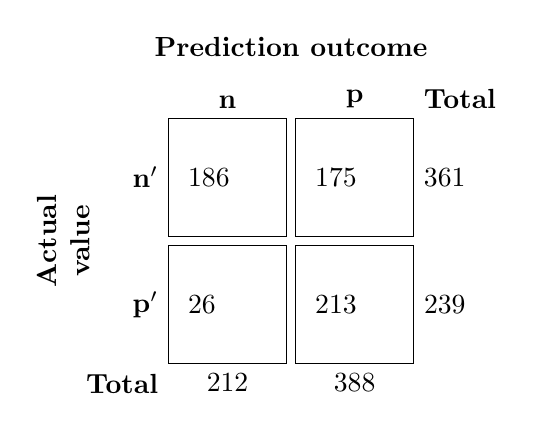
\begin{tikzpicture}[
box/.style={draw,rectangle,minimum size=1.5cm,text width=1.0cm,align=left}]
\matrix (conmat) [row sep=.1cm,column sep=.1cm] {
\node (tneg) [box,
    label=left:\( \mathbf{n'} \),
    label=above:\( \mathbf{n} \),
    ] {186};
&

\node (fpos) [box,
    label=above:\textbf{p},
    label=above right:\textbf{Total},
    label=right:\( \mathrm{361} \)] {175};
\\
\node (fneg) [box,
    label=left:\( \mathbf{p'} \),
    label=below left:\textbf{Total},
    label=below:212] {26};
&
\node (tpos) [box,
    label=right:\( \mathrm{239} \),
    label=below:388] {213};
\\
};
\node [rotate=90,left=.05cm of conmat,anchor=center,text width=1.5cm,align=center] {\textbf{Actual \\ value}};
\node [above=.05cm of conmat] {\textbf{Prediction outcome}};
\end{tikzpicture}
\caption{Confusion Matrix for Testing Dataset Projected to first 3 PCs}
\label{fig:pca}
\end{center}
\end{figure}

This is a major decrease in performance. In an attempt to increase the performance on this projected dataset, the learning rate is dropped to 0.02, the neurons per layer is set at 2, and the number of hidden layers is set to 1. This will simplify the model for the now three dimensional dataset. The confusion matrix for this is shown below, in Figure \ref{fig:pca2}. The accuracy of this run is 69.50\%, with 67.36\% sensitivity, 60.53\% precision, 70.91\% specificity, and a F1 score of 63.76\%.

\begin{figure}[H]
\begin{center}
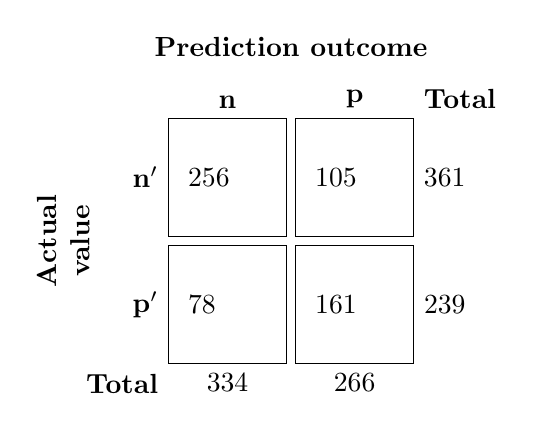
\begin{tikzpicture}[
box/.style={draw,rectangle,minimum size=1.5cm,text width=1.0cm,align=left}]
\matrix (conmat) [row sep=.1cm,column sep=.1cm] {
\node (tneg) [box,
    label=left:\( \mathbf{n'} \),
    label=above:\( \mathbf{n} \),
    ] {256};
&

\node (fpos) [box,
    label=above:\textbf{p},
    label=above right:\textbf{Total},
    label=right:\( \mathrm{361} \)] {105};
\\
\node (fneg) [box,
    label=left:\( \mathbf{p'} \),
    label=below left:\textbf{Total},
    label=below:334] {78};
&
\node (tpos) [box,
    label=right:\( \mathrm{239} \),
    label=below:266] {161};
\\
};
\node [rotate=90,left=.05cm of conmat,anchor=center,text width=1.5cm,align=center] {\textbf{Actual \\ value}};
\node [above=.05cm of conmat] {\textbf{Prediction outcome}};
\end{tikzpicture}
\caption{Confusion Matrix for Testing Dataset Projected to first 3 PCs}
\label{fig:pca2}
\end{center}
\end{figure}

Overall, projection onto the first three principal components did not help the performance of the neural network. Of course, only a very small number of hyper-parameters were tested, and Principal Component Analysis could very well increase overall performance with a specific architecture of the neural network. 

\section{Results}
\label{sec:results}

The performance metrics did not vary much during cross-validation of the hyper-parameters, which makes it difficult to choose optimal values. When choosing the optimal hyper-parameters to reduce false positives, there is an unexpectedly high false positive rate in the testing dataset. To this end, the optimal hyper-parameters chosen are 0.1 learning rate, 2 hidden layers, and 3 neurons per hidden layer (coincidentally, this is the first confusion matrix, Figure \ref{fig:l1}). The first three principals components cover about 99.99\% of the dataset, and the dataset is projected to its first 3 principal components in an attempt to increase performance. Unfortunately, this decreased performance in the testing dataset.

\section{Conclusion}
\label{sec:conclusion}
An artificial neural network is implemented and its hyper-parameters are cross-validated using K-fold cross validation. The performance of each cross-validation did not vary much, and each had a significantly high false negative rate. The neural network is trained on the training dataset with chosen optimal hyper-parameters, and the testing dataset is forwarded through the network, which leads to significantly higher performance metrics than any of the K-fold executions. Performance metrics would likely vary more or even increase if the program was allowed to run further than 1000 epochs. Unfortunately, the complexity of the algorithm makes further testing impractical in the time period of this writing. 


\end{document}

